\section{K-means Clustering}

\subsection{Part 1}
\textbf{Task:} Explain initialization sensitivity and one mitigation strategy.

\paragraph{Answer.}
K-means minimizes the within-cluster sum of squares (WCSS), but this objective is non-convex. As a result, the algorithm may converge to different local minima depending on the initial centroid positions. Two runs with different random starts can therefore produce different cluster assignments and different final WCSS values.

A robust mitigation is \textbf{K-means++ initialization}, which spreads initial centroids by selecting each new centroid with probability proportional to the squared distance from the closest already chosen centroid. This reduces poor starts and generally improves stability. Another standard practice is multiple random restarts and selecting the run with the lowest WCSS.

\subsection{Part 2}
\textbf{Task:} Implement K-means with K=3 and visualize clusters + centroids.

\paragraph{Answer.}
The dataset from \texttt{data\_cluster.csv} was loaded and clustered using a custom NumPy implementation with iterative assignment and centroid update steps until convergence.

For \(K=3\), the final centroids obtained were:
\begin{itemize}
  \item Cluster 0: \([4.9753,\ 6.1344]\)
  \item Cluster 1: \([0.8643,\ 0.9280]\)
  \item Cluster 2: \([8.1211,\ 1.9222]\)
\end{itemize}

The cluster visualization uses color-coded points and explicit centroid markers, with labeled axes and legend for readability.

\begin{figure}[h]
  \centering
  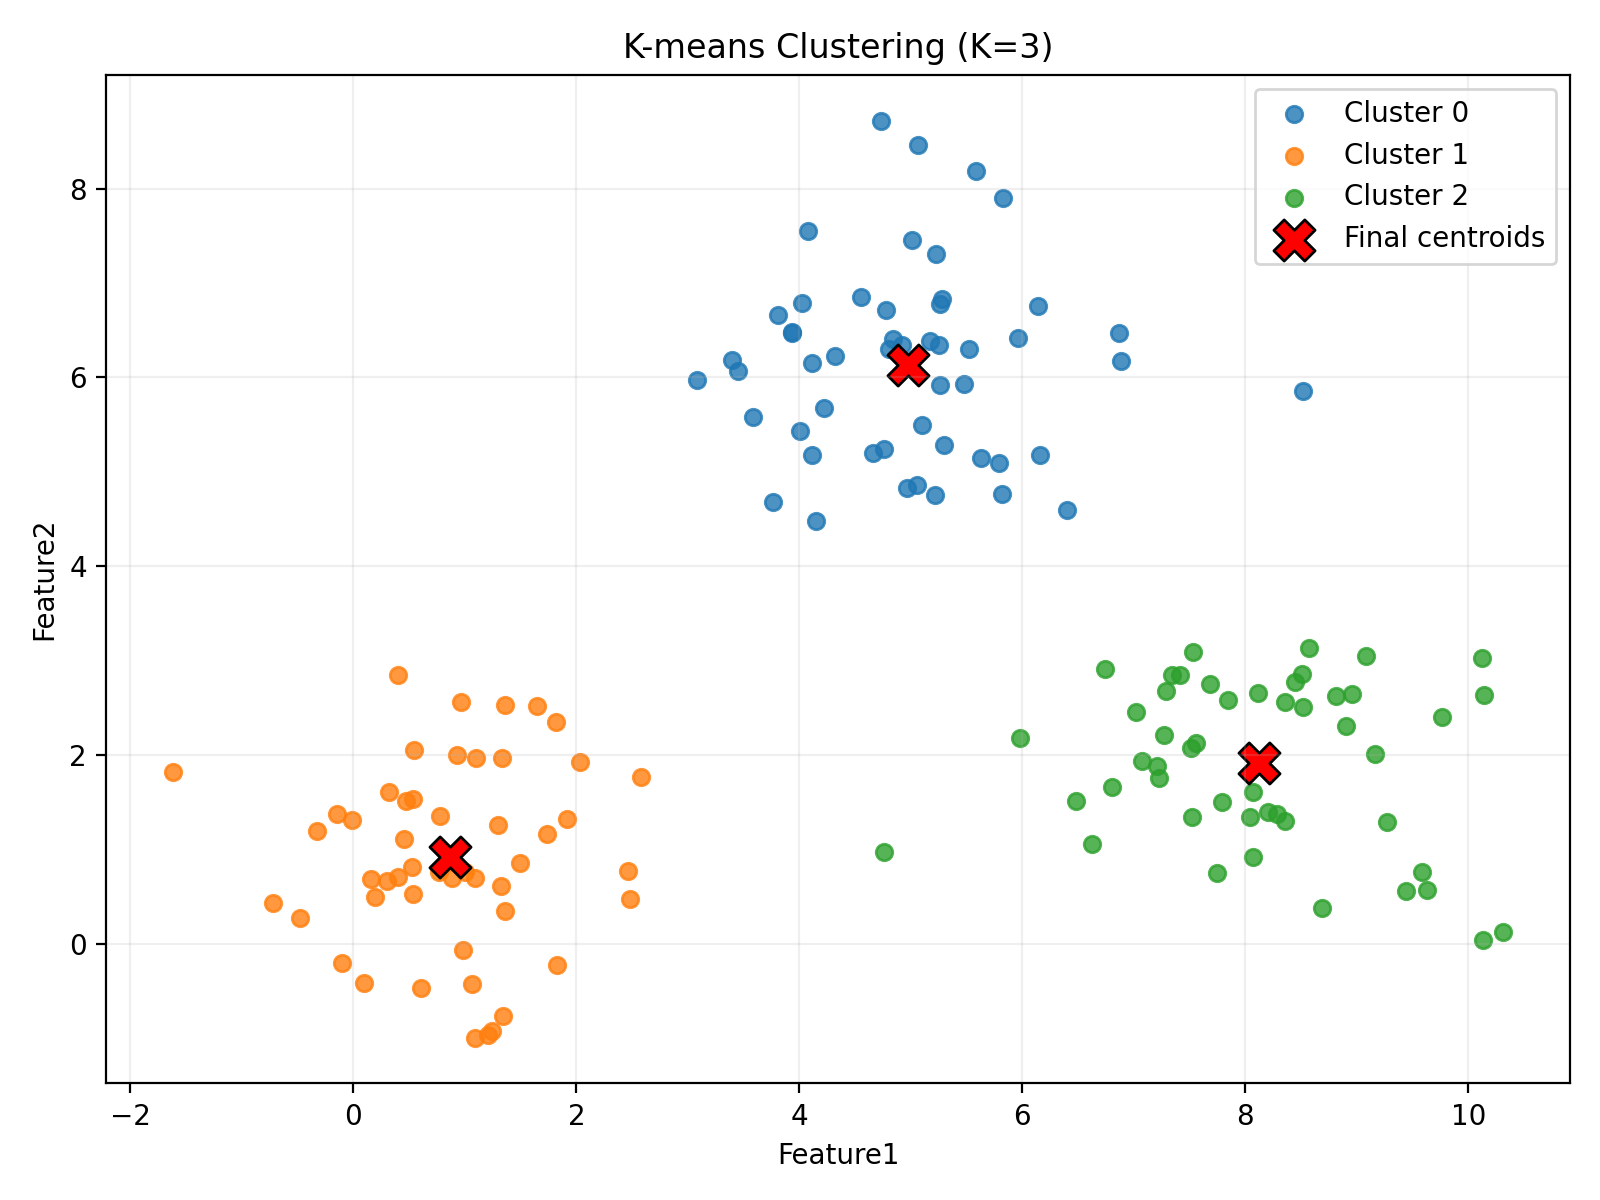
\includegraphics[width=0.75\textwidth]{../K-means/kmeans_clusters.png}
  \caption{K-means clusters for K=3.}
\end{figure}

\subsection{Part 3}
\textbf{Task:} Build elbow curve (K=2..6) and interpret optimal K.

\paragraph{Answer.}
WCSS values for the elbow analysis are:
\begin{center}
\begin{tabular}{cc}
\toprule
\(K\) & WCSS \\
\midrule
2 & 974.4308 \\
3 & 283.7533 \\
4 & 252.0666 \\
5 & 227.9890 \\
6 & 185.4181 \\
\bottomrule
\end{tabular}
\end{center}

The elbow is clearly around \(K=3\): there is a very large improvement from \(K=2\) to \(K=3\), followed by progressively smaller gains for larger \(K\). This aligns with the expected three-cluster structure of the synthetic data.

\begin{figure}[h]
  \centering
  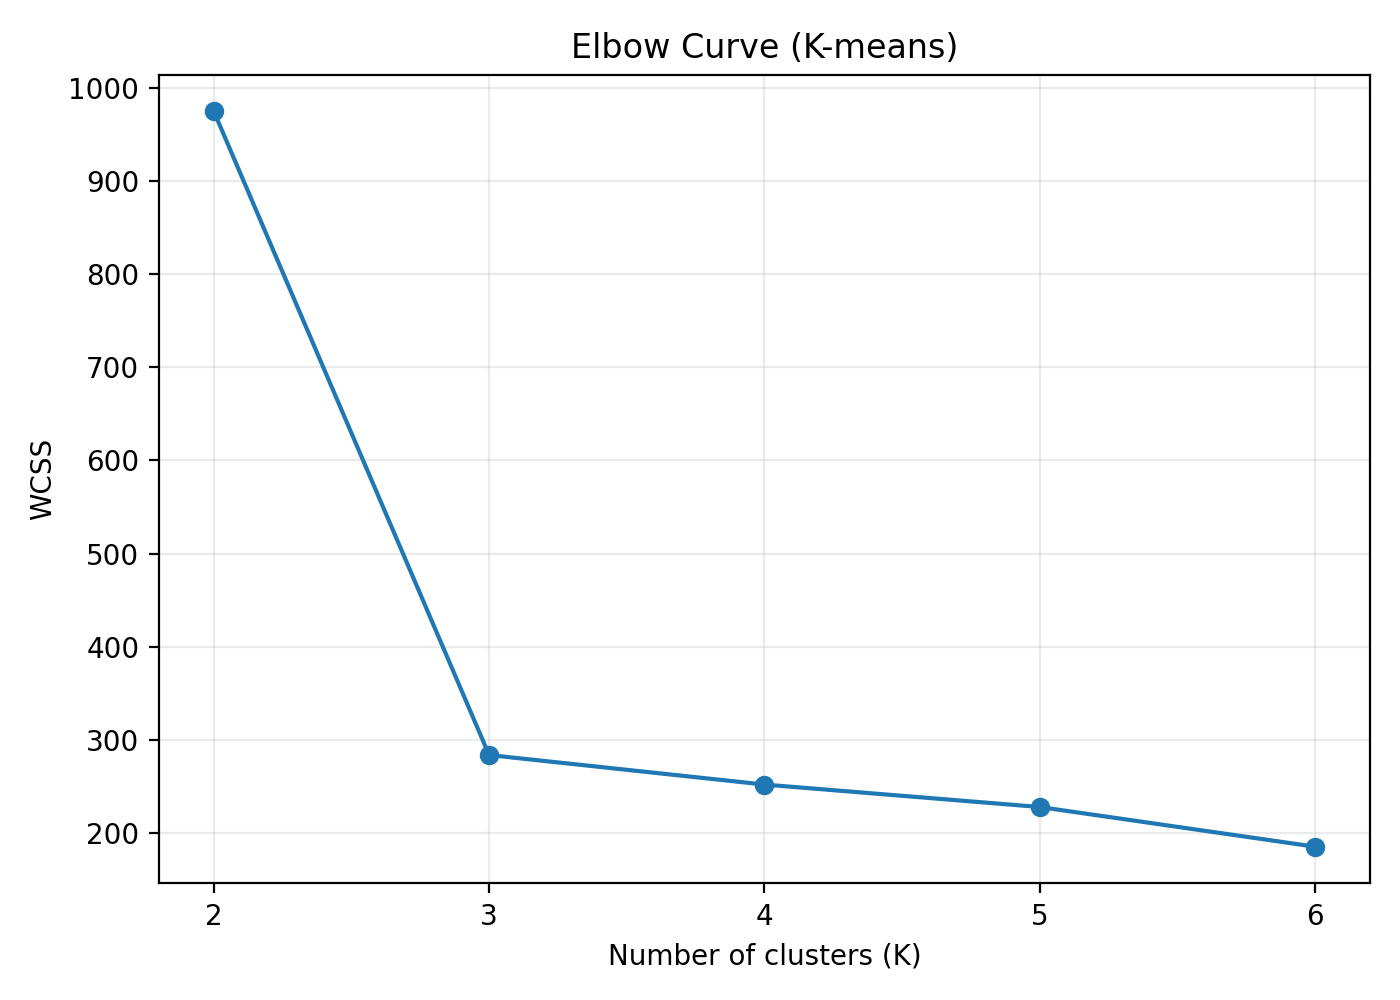
\includegraphics[width=0.75\textwidth]{../K-means/kmeans_elbow.png}
  \caption{Elbow curve for K-means (WCSS vs K).}
\end{figure}

\subsection{Part 4}
\textbf{Task:} Explain WCSS trend with K and discuss initialization effects.

\paragraph{Answer.}
WCSS decreases monotonically as \(K\) increases because additional centroids provide more flexibility: each point can be assigned to an equal or closer center compared to smaller \(K\). Therefore, the minimum achievable WCSS cannot increase when a new cluster is allowed.

To quantify initialization sensitivity, \(K=3\) was tested with seeds \(0\) to \(9\):
\begin{center}
\begin{tabular}{ccc}
\toprule
Seed & Iterations to Converge & Final WCSS \\
\midrule
0 & 4 & 283.7533 \\
1 & 4 & 283.7533 \\
2 & 5 & 943.2848 \\
3 & 4 & 946.9119 \\
4 & 4 & 283.7533 \\
5 & 3 & 283.7533 \\
6 & 4 & 283.7533 \\
7 & 4 & 283.7533 \\
8 & 5 & 283.7533 \\
9 & 4 & 283.7533 \\
\bottomrule
\end{tabular}
\end{center}

Most initializations converge to the best solution (\(\text{WCSS}\approx 283.75\)), but some seeds converge to much worse local minima (\(\text{WCSS}\approx 943\) to \(947\)). This directly confirms the theoretical sensitivity to centroid initialization.
